\chapter{Realizace}
Popis implementace/realizace se zaměřením na nestandardní části řešení.

\section{Průběh realizace}
Průběh realizace jsem si zpětně rozdělil do několika fází, tak jak šly chronologicky po sobě. Každá fáze představuje určitou etapu ve vývoji knihovny.
\\
\\
\noindent Fáze 1

\noindent Po analýze a návrhu byla naimplementována zkušební část kvůli ověření návrhu tříd a rozhraní. Na tuto verzi byla napsána první velká skupina unit testů. Verze nepracovala vůbec s databází, byla pouze instanční a od současného modelu tříd se velmi odlišovala. Tato část práce byla součástí mého softwarového projektu.
\\
\\
\noindent Fáze 2

\noindent Po dokončení instanční verze jsem pokračoval seznámením se s databází eXist-db, která mi byla doporučena vedoucím práce. V této fázi nastaly největší potíže. Nemohl jsem najít způsob, jak komunikovat s databází. V Ruby neexistovalo žádné komunikační rozraní, které by umožňovalo měnit obsah a dotazovat se na něj. Dokumentace přímo na webu \cite{exist:exist} popisovala jenom protokoly, kterými lze s databází komunikovat. Mezi ně patří napríklad REST\footnote{Representational State Transfer}, SOAP\footnote{Simple Object Access Protocol} a XML-RPC, který jsem si zvolil pro vývoj API. Velice mi pomohlo, nalezení ukázky knihovny pro XML-RPC v instalačním adresáři eXist-db. 

Komplikace tím neskončily. Uměl jsem sice pomocí XML-RPC pracovat s kolekcemi a dokumenty, ale nedokázal jsem pomocí xUpdate upravovat dokumenty: vkládat, upravovat a mazat uzly a atributy. Dodržel jsem dokumentaci XML-RPC, specifikace metody \verb|XUpdate| \cite{exist:xmlrpcxupdate} a dokumentaci XUpdate \cite{xupdate}, na kterou se eXist odvolává. V této fázi se mi delší dobu nedařilo zporvoznit upravování dokumentů. Proto jsem začal vyhledávat alternativní možnosti. Hledal jsem XML databázi, která by měla komunikační rozhraní v Ruby. Našel jsem jedinou databázi jménem Sedna. Bohužel ani s ní jsem nedospěl pokroku. Problém byl se zprovozněním knihoven, které byly napsané v jazyku C.

Významnou pomocí v této fázi pro mě byla rada vedoucího mojí bakalářské práce Ing. Strnada, který mě nasměroval na použití technologie xQuery Update Facility.
\\
\\
\noindent Fáze 3

\noindent Přepracoval jsem první verzi implementace RubyACL z lokální/instanční na databázovou, což představovalo přepsání tříd na pseu-singlotonské managery. Třídy nejsou čistými singletony, ale knihovna obsahuje pouze jednu instanci od každé pomocné třídy. Všechny informace jsou uloženy v databázi. RubyACL pouze vkládá nové záznamy, upravuje a maže staré. Na existujících záznamech provádí dotazy a rozhodování o přístupu. Při úplném naimplementování eXistAPI, jsem kompletně předělal třídní model. Do této doby byly třídy jako Principal, Privilege, ResourceObject a ACE používány pro ukládání dat do instancí a polí instancí. Ve fázi 3 jsem tyto třídy předělal na pomocné třídy, které upravují pomocí poskytnutého rozhraní obsah databáze. Přidal jsem třídy Individual a Group. Dalším nezdarem v této části bylo vytvoření nějakého referenčního systému mezi ACL objekty.  Pro identifikaci a propojení jsem uvažoval mezi xLink a idref. Idref nabízí jednoduchý systém, ale xLink nabídl podrobné specifikace W3C, velké množství návodů a turtoriálů a především se jedná o novější technologii, jejíž osvojení jsem považoval za výhodné. Rozhodl jsem se proto implementovat xLink. Problém nastal při některých vkládání textů a dotazování. eXist-db měla problém s jmeným prostorem xLink i přes zkutečnost, že jmený prostor byl uveden jak v samotném XML dokumentu, tak ve vkládaném uzlu. I když jsem se zabýval proč použití xLink nejde, nedospěl jsem rozřešení a tak jsem raději přešel na jednoduchý idref. Implementace idref proběhla rychle a bez problémů.
\\
\\
\noindent Fáze 4

\noindent Druhý návrh tříd nebyl zcela správný a i implementace se odchylovala od návrhu. Znovu jsem musel zasáhnout do modelu tříd a předělat jej. Vytvořil jsem nadřazenou třídu \verb|ACL_Object|, ze které dědí ostatní pomocné třídy. V této fázi jsem velmi intenzivně testoval. Opakované ověřování správné funkčnosti při neustálém upravování knihovny, mi zabíralo příliš mnoho času. V této fázi jsem docenil význam unit testů a jejich schopnost odhalovat chyby.
\\
\\
\noindent Fáze 5

\noindent Dokončil jsem rozhodovací metodu \verb|check| a dotáhl do finální podoby funkcionality knihovny. V této fázi jsem opravil chyby a odstranil nedostatky. Přidal jsem další velkou část unit testů, převážně zaměřených na metodu \verb|check|. Začal jsem tvořit dokumentaci.
\\
\\
\noindent Fáze 6
TODO
\noindent Finalizování - rubygem. Dokumentace. Codecoverage


\section{Programy použité při vývoji}
V následujícím seznamu jsou uvedeny všechny programy, které jsem při vývoji knihovny použil.
\begin{itemize}
\item NetBeans s Ruby platformou od Thomase Enebo
\\
\url{http://blog.enebo.com/}
\\
\url{http://plugins.netbeans.org/plugin/38549/ruby-and-rails}
\item GIT
\url{https://github.com/sirljan/Ruby-ACL}
\item eXist-db
\url{http://www.exist-db.org}
\item Enterprise Architect
\item MikTex
\end{itemize}
%-------------------------------------
\section{Databáze}
Protože XML databáze, která má RubyACL používat, není dosud plně funkční, nebylo možné implementaci testovat přímo na ní. Za tímto učelem se musela vybrat jiná podobná databáze.

\subsection{Sedna}
Databáze Sedna poskytuje rozhraní v Ruby. Klientské rozhraní je Ruby rozšíření, které používá ovladač jazyka C, který je dodáván jako součást distribuce Sedna. Použití má být jednoduché a snadno použitelné. Ovšem zprovoznění knihovny Sedna je nedostatečně popsané a nekompatibilní se současnou verzí Ruby 1.9.3.

\subsection{eXist-db}
Open source systém eXist-db je systém pro správu databáze vytvořené pomocí technologie XML. Databáze eXist-db ukládá XML data podle datového modelu XML a nabízí efektivní a XQuery zpracování založené na indexování. Podporuje velké množství technologií. Dále zde uvádím pouze ty, které se týkají RubyACL nebo eXistAPI: XPath 2.0, XQuery, XML-RPC, XQuery Update Facility 1.0. 

eXist-db se podobá XML databázi, která má RubyACL používat, a byla doporučena vedoucím práce jako ideální. Přesto se vyskytly komplikace s XUpdate navzdory přesné interpretace dokumentace. Z tohoto důvodu bylo nutné přejít na XQuery Update Facility.

\subsubsection{eXistAPI}
ExistAPI je komunikační rozhraní, jehož implementaci si vynutilo ladění a testování knihovny RubyACL na databázi eXist-db. Jednalo se o trochu nestandartní část realizace, protože eXist-db nemá knihovnu rozhraní pro jazyk Ruby.

eXistAPI komunikuje s databází prostřednictvím XML-RPC protokolu a technologíí XQuery a XPath. XQuery Update Facility se používá pro editování dat v dokumentech kolekcí databáze.
Pokus o naimplementování XUpdate nebyl úspěšný. XUpdate není podporován konzorciem W3C\footnote{World Wide Web Consortium} a tudíž není jednoznačně nadefinovaný. Zde nejspíše vznikl problém, kdy eXist-db použila jinou interpretaci XUpdate, než uvádí dokumentace XUpdate \cite{xupdate}.

Interface eXistAPI považuji za přínos pro uživatele eXist-db, kteří programují v Ruby nebo to mají v plánu. Rozhraní eXistAPI je ošetřené vyjímkama, otestované a zdokumentované tak, jak to vyžaduje balíčkovací systém \href{https://rubygems.org/}{RubyGem}, kde ho lze najít pod jménem "eXistAPI". Lze jej tedy stáhnout příkazem \verb|gem install eXistAPI|. Model tříd je v příloze \ref{fig:eXistAPI}. 

%-------------------------------------
\section{Implementace}
V této sekci se zabývám popisem implementace metody \verb|check| a rozepsaní a popsání příkladu založení uživatele.

\subsection{Třída RubyACL}

Hlavní účel třídy \verb|RubyACL| je zprostředkovávat funčnost pomocných tříd dědících z třídy \verb|ACL_Object|. Dále sama nabízí možnost ukládání a načítání ACL ze souborů a hlavně obsahuje metodu \verb|check|, která slouží k vyhodnocování pravidel.

\subsubsection{Metoda check}
Metoda check obsatarává rozhodování, jestli zmocnitel má oprávnění k objektu nebo nemá. Stručně a výstižně vysvětluje algoritmus obrázek \ref{fig:check}. 

Metoda \verb|check| nejprve zjistí, jestli daný zmocnitel není vlastník daného objektu nebo jakéhokoliv nadřazeného objektu. Pokud je ihned vratí true a ukončí běh. 
Pokud zmocnitel není vlastníkem, metoda \verb|check| nashromáždí všechny potenciální pravidla, která by mohly ovlivňovat přístup. Udělát to tak, že pro daného zmocnitele najde všechny jeho nadřezené zmocnitele. Jedná se tedy o pole skupin a pokud je daným zmocnitelem jednolivec, tak i on. Obdobným způsobem vytvoří i pole privilegií a nadřazených privilegií. zdojových objektů a nadřazených zdrojových objektů. Dále z těchto polí vytvoří XQuery dotaz, který vybere takové pravidlo, které obsahuje jednoho ze zmocnitelů a zárověn jedno z pravidel a zároveň jeden zdrojový objekt. XQuery se odešle pomocí eXistAPI a přijme se množina pravidel. V této množině pravidel hledá metoda \verb|check| pravidlo, které má nejvyšší prioritu. Metoda určuje prioritu podle seznamu v sekci \ref{Priorita rozhodování} Priorita rozhodování. Metoda prochází pravidla a srovnává pravidlo uložené ve pomocné proměnné s aktuálním pravidlem. Pokud aktuální má větší prioritu zapíše ho do pomocné proměnné. Pokud není žádný další záznam, metoda přečte \verb|accessType| a podle něj rozhodne, co vrátí. Pokud \verb|accessType| obsahuje "allow" vrátí true, pokud obsahuje "deny" vrátí false.
\begin{figure}
%\centering
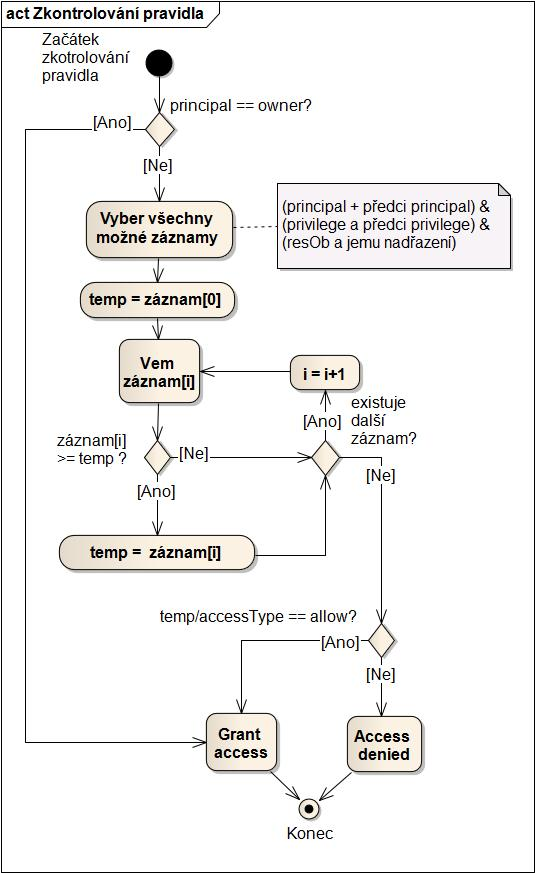
\includegraphics[width=15cm]{check2.jpg}
\caption{Diagram znázorňující chod metody check}
\label{fig:check}
\end{figure}

\subsubsection{Příklad}
Uvedu zde jeden příklad vytvoření zmocnitele a na něm vysvětlím TODO.

\lstset{language=Ruby, numbers=none}
\begin{lstlisting}
@my_acl.create_principal("Sheldon", "4th_Level")
\end{lstlisting}

Je zřejmé, že příkaz volá metodu \verb|create_principal|. Příkaz má vytvořit zmocnitele jménem \verb|"Sheldon"|, který bude patřit do skupiny \verb|"4th_Level"|. RubyACL má instanci od každé pomocné třídy. RubyACL tedy pouze zavolá metodu \verb|create_new| instance @indi, což je instance třídy Individual. Metoda \verb|create_new| ničím nekonkrétizuje chování supertřídy \verb|ACL_Object|, takže se zavolá metoda této třídy. Zde se provede kotrola, jestli jméno není prázdné. Pokud jméno je prázdné vyhodí se vyjímka. Dále se pokračuje kontrolou, jestli jméno už není obsazené. Pokud je, vyhodí se vyjímka. Pomocí metody \verb|generate_expr| se vygeneruje uzel, který bude následně skládat. Metoda \verb|generate_expr| není ve třídě Individual přepsaná (anglicky overriden), takže se v tomto případě volá metoda supertřídy. Výsek kódu tvoření uzlu je v následujícím výpisu:

\begin{lstlisting}
    expr = <<END
    <#{self.class.name} id="#{name}">
      <membership>
        
      </membership>
    </#{self.class.name}>
END
\end{lstlisting}
Kód ukazuje, že jméno uzlu je utvořeno podle jména třídy (jedná se o část \verb|self.class.name|), takže jméno uzlu je v tomto případě "Individual". Dalším krokem je vytvoření části příkazu, který rozhoduje kam se uzel bude vkládat a opět se využívá jména třídy.
\begin{lstlisting}
expr_loc = "#{@doc}//#{self.class.name}s/#{self.class.name}[last()]"
\end{lstlisting}
Zbývá už pouze zavolat metodu \verb|update_insert| instance třídy eXistAPI, která vloží připravený uzel na připravenou pozici. Následně se zkontroluje, pokud byl uzel vložen, pokud ne, vyvolá se vyjímka.

Následuje větvení, které rozhoduje zda se bude zmocnitel přidávat do nějaké skupiny. V tomto případě se zmocnitel do skupiny bude přidávat. Přidávání se provádí pomocí metody \verb|add_membership|, kterou lze volat i samostnatně. Parametry metody jsou: "kdo má být", "v jaké skupině". Metoda zjednodušeně řečeno vkládá do zmocnitele odkaz na skupinu. \verb|add_membership| funguje podobně jako \verb|create_new| - připraví se uzel na vkládání, připraví se lokace vložení jako XPath výraz a předtím než se zavolá \verb|update_insert| se zkontruluje, jestli se členství necyklí. Nakonec se zkontroluje, pokud byl uzel vložen, pokud ne, vyvolá se vyjímka.


%-------------------------------------

\subsection{ACL\_Object}
Třída \verb|ACL_Object| je rodičem tříd: Principal, Privilege, ResrouceObject, ACE a nepřímým rodičem Individual a Group.
Třída sdružuje obecné metody, které jsou společné pro všechny výše vyjmenované třídy. Takové metody například jsou: \verb|create_new|, \verb|delete|, \verb|rename|. \\ \verb|ACL_Object| také obsahuje důležitou proměnou \verb|doc|, která obsahuje cestu k datovému dokumentu v databázi. Tuto proměnou taktéž třídy dědí.
Jednolivé třídy vyjmenované v této sekci pracují se svým dokumentem. Dokument a uzly v něm mají různou strukturu. Například oprávnění má jeden kořenový uzel a pak už jen list oprávnění, ve kterých jsou odkazy na nadřazené oprávnění. Čili se jedná o poměrně jednoduchou strukturu. Každá ze tříd má tuto strukturu v sobě uloženou a podle ní tvoří dotazy na editování dat.

%-------------------------------------

\subsection{Vyjímky}
Vyjímky pro knihovnu RubyACL vyvolává třída \verb|RubyACLException|. Knihovna buď vyjímky vyvolává nebo je jen propaguje dále. Seznam vyjímek, jejich kódů a metod, které je vyvolávají jsou vypsané v příloze TODO \ref{} a na přiloženém CD přímo pod zdrojovým kódem třídy \verb|RubyACLException|.

Vyjímky pro rozhraní eXistAPI vyvolává třída \verb|ExistException|.

%-------------------------------------

\subsection{Práce s pamětí}
Na začátku mi bylo jasné, že bych neměl zanedbat práci s pamětí, protože aplikace s knihovnou bude spuštěna v řádech dnů a měsíců. Špatné zacházení s pamětí by, proto bylo kritické pro server, na kterém aplikace s Ruby-ACL knihovnou bude spuštěna. Ruby-ACL veškeré data ukládá do databáze. Jediné obsazení paměti je instancí samotné třídy \verb|RubyACL| a instancemi pomocných tříd. Nicméně v Ruby uvolňování paměti programátorem nemá význam, protože v dynamickém prostředí Ruby se o uvolňování stará garbage collector. Ruby používá garbage collector, který nepoužívané objekty vystopuje a odstraní \cite{Ruby}.